The Unidad Popular's electoral victory in 1970 brought a programme of socialist transformation into contact with social forces that had been reorganizing Chilean society for several decades. Industrial workers, rural laborers, \emph{pobladores}, students, and sections of the urban middle classes did not enter the political scene at the same moment or through the same institutions. Their demands were rooted in different locations of the economy and in different experiences of the developmental state. What gave the Popular Unity coalition its historical depth was the gradual convergence of conflicts around work, land, urban residence, and social rights. This section reconstructs that convergence as four waves of social conflict. Throughout, these historical waves must be distinguished from the accounting windows used in the empirical analysis: the waves describe historical political periods, whereas the profitability decompositions in Tables~\ref{tab:profitability_decomposition} and \ref{tab:accumulation_accounting} begin later and are bounded by annual data availability.

The economic background to these conflicts reaches back before the Great Depression. Chile entered the twentieth century as an export economy centered on nitrates, with mineral rents financing a large share of public revenue and sustaining commercial, fiscal, and urban expansion. This export boom also generated domestic demand. Public expenditure, mining settlements, transport networks, and the growth of Santiago, Valpara\'{\i}so, and other cities enlarged the market for locally produced manufactures. A meaningful manufacturing sector thus emerged well before state-led import substitution became an explicit development strategy. On the eve of the First World War, manufacturing represented roughly one-seventh of Chilean output, though concentrated primarily in food, beverages, textiles, clothing, and other simple consumer goods \citep{BulmerThomas2003}. This was industrial growth nested within an export economy rather than an autonomous industrial take-off.

In older historiography, the international disruptions beginning in 1914 were often treated as the decisive stimulus to domestic manufacturing \citep{Palma1984}. The newer reconstruction by P\'erez-Eyzaguirre substantially qualifies that interpretation. His revised series shows that Chilean industrial production had expanded alongside the export economy prior to 1914 and then contracted sharply when the war disrupted trade, imported inputs, and capital flows. Under this reconstruction, the level of industrial production achieved in 1913 was not recovered until 1941 \citep{PerezEyzaguirre2025}. The war exposed how strongly domestic manufacturing still depended on the commercial and financial circuits generated by primary exports, rather than initiating an uninterrupted wartime industrial boom.

Urbanization followed an equally distinctive trajectory. Chile was already highly urbanized by Latin American standards prior to the classic period of state-led industrialization. P\'erez-Eyzaguirre estimates that 46.7 percent of the population lived in urban settlements by 1930, emphasizing that the nineteenth- and early twentieth-century urban transition was tied more closely to export expansion, state formation, and successive primary-export cycles than to manufacturing employment alone \citep{PerezEyzaguirre2017}. This urban transition shaped subsequent labor politics: an urban population, an expanding state apparatus, and a domestic market formed before industry could absorb the majority of workers leaving rural activities. Chile entered the Depression with an unusually urban social structure relative to the productive apparatus supporting it.

The collapse after 1929 transformed these inherited tensions into a crisis of the existing accumulation pattern. Chile was among the Latin American economies most exposed to the contraction of world trade: the purchasing power of exports fell by roughly four-fifths during the first years of the Depression, while aggregate output fell dramatically between 1929 and 1932 \citep{BertolaOcampo2012,BulmerThomas2003}. Between 1929 and 1932, recorded employment fell from 1.43 million to 1.17 million workers, a loss of roughly 262,000 jobs, or 18 percent of the 1929 employment level. Over the same interval, measured unemployment increased from about 34,000 to 374,000 workers in the historical series used in this paper, raising the unemployment rate from 2.35 to 24.30 percent. Beyond the immediate loss of national income, the collapse sharply contracted the foreign-exchange flows around which fiscal revenue, imports, mining demand, transport, commerce, and much of the domestic market had been organized. Restoring economic activity required a fundamentally different relation between the state, domestic demand, and production.

The initial policy response was pragmatic. Under Arturo Alessandri's second administration (1932--1938), deficit spending, public works, industrial credit, exchange controls, and tariff protection were deployed to reactivate employment and domestic production. As \citet{Silva2007} emphasizes, import substitution emerged during this stage through crisis management before crystallizing into a coherent developmental model. Emergency state intervention reorganized accumulation before the institutional machinery of the later developmental state was established. Industrial policy remained compatible with agrarian interests, supporting branches such as food processing and leather that were directly linked to domestic agriculture. This compatibility explains why early restructuring attracted joint support from financiers, merchants, landowners, and industrialists without requiring an immediate political rupture between an industrial bourgeoisie and a landed oligarchy.

Sources of growth between 1929 and 1939 reflect this structural redirection. For Chile over this decade, B\'ertola and Ocampo estimate that import substitution contributed approximately 1.3 percentage points per year to growth, while the contributions associated with domestic demand and exports were slightly negative, yielding aggregate output growth of only about 0.8 percent per year \citep{BertolaOcampo2012}. Domestic production substituted for imports while the external and domestic demand components inherited from the nitrate regime remained depressed. Manufacturing recovered much faster than aggregate activity, averaging roughly 7.7 percent annual growth between 1932 and 1939 \citep{BulmerThomas2003}---a trajectory of structural import substitution distinct from simple cyclical recovery.

The Popular Front victory in 1938 accelerated this transformation into a second stage. The creation of CORFO in 1939 provided the state with an institutional vehicle for economic planning, infrastructure provision, public enterprise, and the long-term financing of strategic industries. The expansion of electricity, steel, fuels, transport, and intermediate inputs widened the productive base beyond the light consumer branches inherited from the export era. Under CORFO's coordination, industry's share of GDP rose from approximately 13 percent in 1940 to roughly 21 percent in 1950 \citep{Silva2007}. During the Second World War, Chilean industrial output expanded much faster than aggregate GDP, consolidating manufacturing growth while world trade was disrupted \citep{BulmerThomas2003}. By 1950, manufacturing represented roughly a quarter of Chilean GDP in the B\'ertola--Ocampo estimates, exceeding the Latin American average \citep{BertolaOcampo2012}. The postwar economy was substantially more industrial than the economy that had entered the Great Depression.

The consolidation of Chilean import substitution coincided with the construction of what regulation theory identifies as Atlantic Fordism. In the United States and Western Europe, mass production was embedded in national growth regimes based on mass consumption, collective bargaining, Keynesian demand management, and welfare-state institutions, while Bretton Woods provided an international monetary framework compatible with national policy autonomy \citep{Vidal2015,Vidal2019}. Much of this Golden Age growth remained organized around domestic and regional mass markets rather than unrestricted global product-market competition.

The internationalization of this accumulation regime did not imply that peripheral economies reproduced the institutional architecture of the Fordist core. As \citet{Cardoso1972} emphasized in his analysis of the new forms of dependency, postwar foreign capital increasingly entered industrial production itself, often in combination with local private and state capital. Industrialization and structural dependency advanced together: while domestic manufacturing deepened, the reproduction of productive capacity remained asymmetrical because advanced technology and the production of means of production remained concentrated in the core capitalist economies. Dependent industrialization thus required external complementarity to complete its accumulation process, even as Latin America's share of world trade fell from 12 percent in 1948 to 6 percent in 1968 \citep{Cardoso1972}.

Chile's developmental trajectory was therefore a peripheral adaptation to the North Atlantic Fordist order rather than a domestic replica of Fordism. Industrial capacity expanded, but its reproduction deepened dependence on imported capital goods, intermediate inputs, replacement parts, foreign technology, and external finance. In his contemporary diagnosis of the early CORFO national accounts, \citet{Kaldor1959} observed that gross fixed-capital formation had only occasionally exceeded 10 percent of GNP after 1940, with more than half of domestic investment undertaken by the public sector. His estimates demonstrated that imported capital goods accounted for roughly two-fifths of fixed investment across the benchmark years examined. The external constraint had moved deeper into the production process itself.

Kaldor also identified an internal bottleneck central to Chilean accumulation: agriculture. Industrial output, non-agricultural employment, and urban incomes expanded faster than the domestic supply of food. Under these conditions, rising demand for wage goods exerted persistent upward pressure on food prices, which fed into wage demands and industrial operating costs. Kaldor treated agricultural stagnation, concentrated landholding, and low rural investment as an integral part of the same accumulation problem as industrial growth \citep{Kaldor1959}. The structural burden of sustaining basic infrastructure and capital formation fell disproportionately onto the state in the face of sluggish private domestic accumulation.

The social transformation generated by industrialization was decidedly uneven. Urbanization advanced faster than factory employment. Between 1940 and 1970, tertiary activities absorbed the largest share of net labor-force growth, while manufacturing and construction combined absorbed a considerably smaller share; the fact that positive sectoral contributions sum to more than 100 percent reflects the absolute contraction of primary-sector employment over the interval. By 1970, in an economically active population of about 3.2~million, \citet{DeVylder1976} counted roughly 260,000 openly unemployed workers and another 600,000 in low-productivity service activities. The city thus became the site where incomplete labor absorption, informal service employment, housing deficits, and unequal access to municipal infrastructure were systematically reproduced.

Chilean industrialization was disarticulated not because it failed to expand manufacturing, public employment, or basic infrastructure, but because productive capacity, labor absorption, and social incorporation proceeded at starkly uneven tempos. In 1970, 87.3 percent of rural dwellings and 26.8 percent of urban homes still lacked piped potable water \citep{DeVylder1976}. The state expanded education, healthcare, and social security while presiding over an unequal geography of incorporation. Migrants entered cities where social services and citizenship were materially more accessible than under the rural estate, even as stable factory employment and adequate housing remained scarce.

Rather than a rigid dichotomy between ``feudal'' estates and ``capitalist'' cities, the Central Valley hacienda had long combined commercial production for national and world markets with concentrated extra-economic control over tenant labor (\emph{inquilinaje}) \citep{Kay1980}. The gradual erosion of these agrarian relations released labor, altered the composition of the working class, and shifted the geographical terrain of collective mobilization without eliminating an urban labor reserve.

Four successive waves of social mobilization and state containment structured this developmental period. These waves track shifts in popular organization, the spatial locus of protest, and state responses. While macroeconomic profitability, capital accumulation, and employment bounded the material space in which disputes unfolded, political organization and state institutions decisively shaped how distributional pressures translated into collective action.

\begin{figure}[H]
\centering
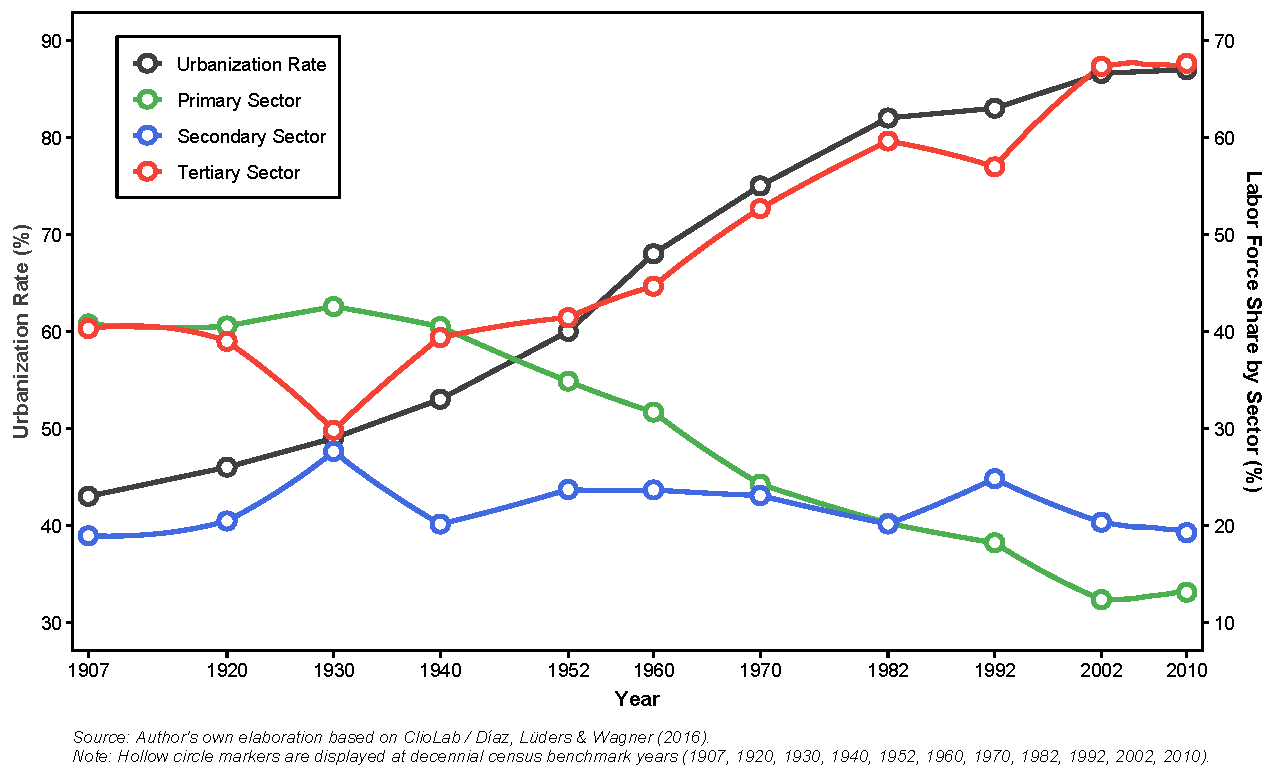
\includegraphics[width=0.90\textwidth]{figures/sec51/fig06_urbanization_labor_sectors.pdf}
\caption{Sectoral labor-force composition and urbanization in Chile, 1907--2010.}
\label{fig:sec51_urban_labor}
\begin{minipage}{0.90\textwidth}\footnotesize
\textit{Source:} Author's elaboration from Clio-Lab PUC historical statistics \citep{DiazLudersWagner2016}. Sectoral series refer to the labor force; urbanization refers to population. These measures have different denominators. Census urbanization observations are plotted as points.
\end{minipage}
\end{figure}

\paragraph{Wave I: Selective incorporation and coercive backlash, 1932--1947.}
The first wave emerged during the reconstruction of the 1930s and reached its crest in the mid-1940s. The 1931 Labor Code established a national framework for collective organization, but incorporation was highly uneven. Urban unions gained a recognized place in industrial relations and electoral politics, while agricultural workers remained subject to estate-level authority and legal restrictions \citep{Milos2008,Loveman1976}. The developmental state expanded productive and social capacities while preserving a differentiated labor regime between city and countryside.

This tension was visible from the beginning. The collapse of the export economy produced unemployment on a scale that weakened labor's immediate bargaining position, but it also destabilized established relations of authority. Rural workers and \emph{inquilinos} used petitions, strikes, and clandestine organization to demand statutory wages, written contracts, and security of tenure. The Ranquil conflict of 1934 exposed the coercive limits of incorporation in the countryside. Under the Popular Front, Communist and Socialist organizers intensified efforts to organize rural labor even as coalition governments remained cautious about confronting landowners directly \citep{Loveman1976}.

By the mid-1940s, rural mobilization converged with renewed industrial militancy. The Plaza Bulnes massacre and the general strikes of January and February 1946 marked the urban-industrial crest of this wave \citep{BravoVargas2017}. Registered agricultural petitions also rose sharply and reached their maximum in 1947 in the series assembled from Loveman's archival evidence (Figure~\ref{fig:sec51_petitions}). This is one reason the 1943--1947 profitability window in Table~\ref{tab:profitability_decomposition} should not be mistaken for the beginning of the wave: it captures the final observed segment of a conflict that had been building since the 1930s.

Distributional accounts are consistent with this tightening conflict. During 1943--1947, a declining profit share ($-5.53$ percent per annum) accounted for the primary negative contribution to profit-rate growth in the paper's decomposition (Table~\ref{tab:profitability_decomposition}). While this pattern demonstrates that workers were gaining distributional ground in the observed interval, it reflects rather than explains the underlying political mobilization.

The state responded through legal segmentation and political repression. Law 8,811, enacted in July 1947, recognized agricultural unions while confining them to individual \emph{fundos}, restricting the seasonal timing of petitions, and imposing eligibility rules that blocked organization across estates \citep{Chile1947}. The following year, Law 8,987 outlawed the Communist Party and excluded targeted militants from electoral and union activity \citep{Chile1948}. These measures did not resolve rural grievances; they suppressed the organizational channels through which those grievances had been articulated.

The closure of rural organization altered the geography of conflict. Migration to urban centers was driven by structural factors predating the late 1940s repression, but the combination of agrarian stagnation, restricted rural organization, urban industrial concentration, and expanding municipal services made cities central to popular politics.

\begin{figure}[htbp]
\centering
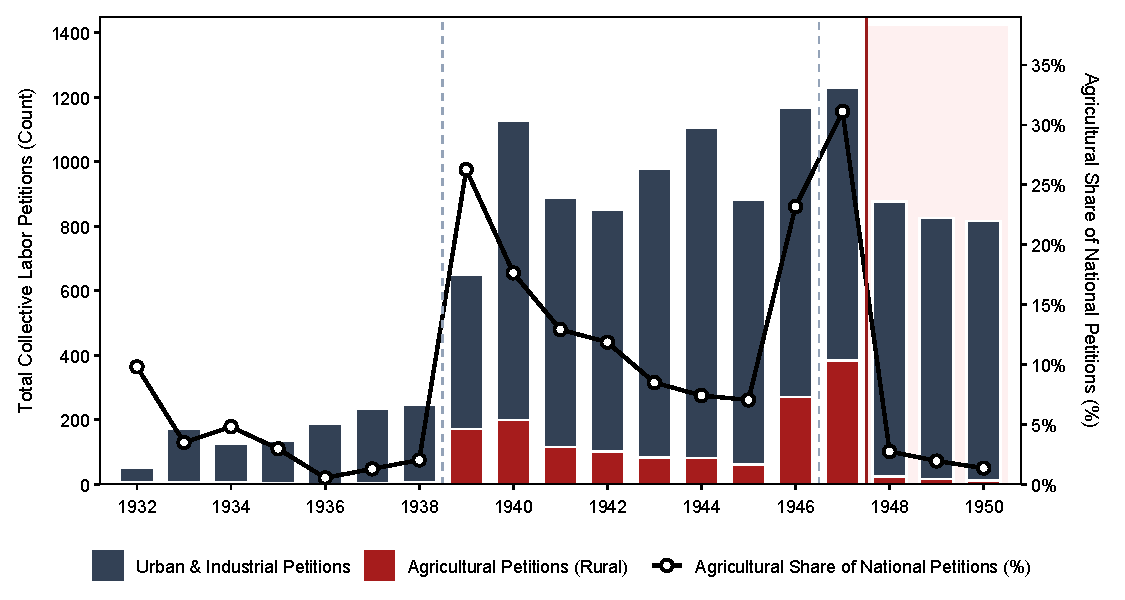
\includegraphics[width=0.88\textwidth]{figures/sec51/fig00_labor_petitions_composition_1932_1950.pdf}
\caption{Recorded collective labor petitions by sector, 1932--1950.}
\label{fig:sec51_petitions}
\begin{minipage}{0.88\textwidth}\footnotesize
\textit{Source:} Author's archival compilation from \citet{Loveman1976}. Petitions measure registered collective demands under the prevailing legal framework, not all forms of social conflict.
\end{minipage}
\end{figure}

\paragraph{Wave II: Coercive containment and urban recomposition, 1948--1958.}
The second wave was defined less by the disappearance of conflict than by its containment and relocation. The restrictions introduced in 1947--1948 narrowed legal space for rural and left organization. During the Ib\'a\~nez administration, the stabilization programme associated with the Klein--Saks mission added statutory wage restraint, credit contraction, and price increases on public transport and foodstuffs. Real wages fell sharply in the mid-1950s while inflation accelerated, shifting the costs of stabilization onto wage earners through workplace discipline and household consumption.

The profitability decomposition documents the distributional consequences of this containment. Between 1948 and 1958, a rising profit share ($+3.11$ percent per annum) provided the largest positive contribution to profit-rate growth ($+2.93$ percent per annum, Table~\ref{tab:profitability_decomposition}), while capital deepening ($-2.60$ log points) offset gains in potential labor productivity ($+2.29$ log points). Distribution shifted toward capital even as industrial and urban transformation continued.

Urban society, however, became more difficult to contain. Industrialization and public investment drew migrants toward the cities without providing factory employment or adequate housing on a commensurate scale. Rather than forming an inert residual of incomplete industrialization, urban neighborhoods became autonomous centers of collective action where migrants, factory workers, informal wage earners, and women organized around transport tariffs, food prices, housing, clinics, and municipal utilities.

In April 1957, protests over transit fare hikes erupted into a nationwide urban revolt, met by military suppression in Santiago, Valpara\'{\i}so, and Concepci\'on. In October 1957, organized families occupied land south of Santiago to establish the \emph{poblaci\'on} La Victoria. Pobladores did not merely petition the state for housing; they occupied land, organized settlement committees, constructed basic infrastructure, and negotiated collectively with public authorities \citep{Garces2002,Murphy2015}. While social conflict is sometimes characterized as having simply shifted from countryside to city, rural grievances persisted alongside industrial unionism and an emerging pobladores movement. What changed was the density of organizational ties linking these arenas.

\paragraph{Wave III: The Long Sixties and the rise of the Unidad Popular, 1959--1970.}
The Long Sixties transformed that urban and rural recomposition into a broader cycle of mobilization. Industrial workers expanded their demands beyond wages toward workplace control, challenging managerial authority over production quotas, safety, and the labor process. Inter-industry solidarity deepened through major conflicts, including the support of Huachipato steelworkers for the 1960 Lota coal strike, while state violence, such as the 1966 killings at the El Salvador copper mine, radicalized union federations \citep{Thielemann2018}.

In the countryside, the Agrarian Reform Law (Law 16,640) and the Rural Unionization Law (Law 16,625) enacted in 1967 dismantled the estate-bound restrictions of Law 8,811, recognizing communal unions and provincial confederations \citep{Chile1967}. Agricultural union membership expanded from 1,658 workers across 24 unions in 1964 to 127,680 members across 488 unions by mid-1970 \citep{DeVylder1976}. Across the economy as a whole, national union density over employed workers doubled from 11.2 percent in 1964 to 22.9 percent by 1970 \citep{OsorioPolanco2021} (Figure~\ref{fig:sec51_wageshare_unionization}). The organizational infrastructure of labor had become dense enough to coordinate action across sectors and regions.

Simultaneously, \emph{pobladores} expanded the politics of social reproduction beyond the wage relation. Land occupations, neighborhood committees, and demands for clinics, schools, transport, water, and paved roads turned access to the city into a field of collective bargaining with the state \citep{Garces2002,Murphy2015}. In centers such as Concepci\'on, industrial unions, student federations, and neighborhood assemblies coordinated strike support and shared logistical resources \citep{Schlotterbeck2018}. The popular movement supporting the Unidad Popular was an articulation of differentiated organized constituencies forged through the uneven development of the period.

Distributional mobilization unfolded within an expanding rather than a contracting economy: across the 1959--1970 accounting interval, the profit rate rose from 8.16 percent to 12.23 percent, supported by positive contributions from the profit share, capacity utilization, and potential labor productivity (Table~\ref{tab:profitability_decomposition}). Sustained accumulation, a larger urban labor force, and denser institutional networks expanded workers' capacity to press claims on national income, property, and state policy.

While a Kaleckian political mechanism links sustained high employment to weakened labor discipline, Chile had not attained generalized full employment. The sectoral and institutional dynamic was decisive: tighter conditions in unionized industries and rising national union density bolstered workers' collective bargaining power even while an informal reserve army persisted in peripheral services.

\begin{figure}[htbp]
\centering
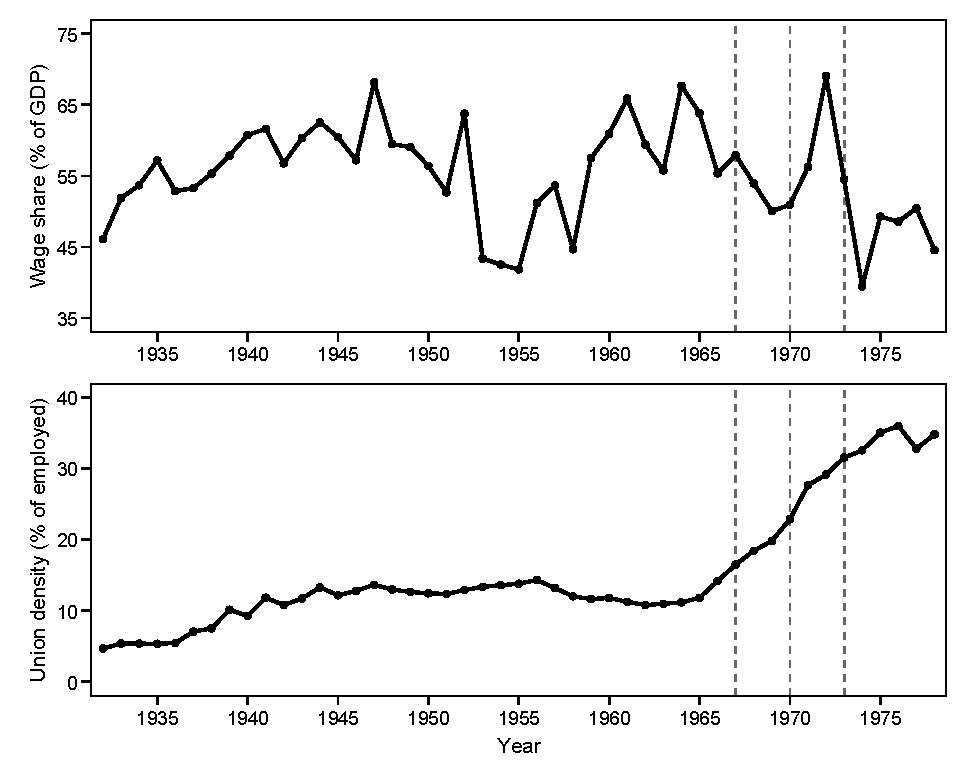
\includegraphics[width=0.88\textwidth]{figures/sec51/fig07_wageshare_unionization.pdf}
\caption{Wage share and unionization in Chile, 1932--1978.}
\label{fig:sec51_wageshare_unionization}
\begin{minipage}{0.88\textwidth}\footnotesize
\textit{Source:} Author's elaboration from \citet{Astorga2023} for Panel~A and \citet{OsorioPolanco2021} for Panel~B. Panel~A reports the functional wage share ($W/Y$, percent of GDP). Panel~B reports union density over employed workers. Vertical dashed lines mark the 1967 agrarian reform and rural unionization statutes (Laws 16,640 and 16,625), the September 1970 election of Salvador Allende, and the September 11, 1973 military coup.
\end{minipage}
\end{figure}

\paragraph{Wave IV: The UP administration and the crisis of accumulation, 1970--1973.}
Allende's election in September 1970 linked these popular movements directly with executive power. The UP programme connected income redistribution to the nationalization of strategic mineral resources, expansion of the social property area, agrarian expropriation, and structural planning. Yet the organizations forged during the preceding waves did not become passive extensions of government. Factory requisitions, land occupations, and community distribution networks frequently pushed ahead of the executive's statutory timetable \citep{Winn1986,Winn2016,Schlotterbeck2018}, generating dynamic tension between state policy and autonomous popular mobilization.

The administration's first year produced an exceptionally large distributive expansion. Real employee remuneration rose by 54.9 percent in 1971 following statutory wage adjustments \citep{DeVylder1976}, and the wage share rose from 50.9 percent of GDP in 1970 to 69.0 percent in 1972 \citep{Astorga2023}. The growth-accounting decomposition reveals a severe initial profit squeeze: the profit rate fell from 12.23 percent in 1970 to 6.57 percent in 1972, while the net accumulation rate declined from 4.23 to 1.85 percent and gross accumulation from 11.63 to 7.64 percent (Table~\ref{tab:accumulation_accounting}). The profit share accounted for most of this decline between 1971 and 1972 (Table~\ref{tab:profitability_decomposition}, Panel~B).

That initial distributive squeeze cannot be projected mechanically over the full three-year interval. Across 1971--1973, relative capital prices ($-4.35$ percent) and capacity utilization ($-4.78$ percent) provided the dominant negative contributions to profit-rate growth, while the contribution of the profit share changed sign (+1.94 percent, Table~\ref{tab:profitability_decomposition}, Panel~A). The annual accounts for 1973 make this divergence evident: the measured profit rate rebounded from 6.57 percent in 1972 to 9.12 percent in 1973, yet net capital accumulation slowed further to 1.71 percent (Table~\ref{tab:accumulation_accounting}). Because annual 1973 data aggregate the final eight months of the UP with the first four months of military dictatorship, they cannot separate pre-coup strikes from post-coup wage repression. They nevertheless demonstrate that profitability alone cannot explain the collapse of capital accumulation.

The terminal crisis concentrated contradictions that had accumulated across multiple decades: an industrial base dependent on imported capital goods and foreign finance; agrarian stagnation that generated wage-good bottlenecks; incomplete urban labor absorption; and a densely organized popular movement capable of mounting structural challenges to property and state authority.

The Unidad Popular concentrated rather than initiated these contradictions. Its redistributive programme accelerated popular mobilization within external and productive boundaries inherited from the developmental era. The next section examines the balance-of-payments constraints and monthly macroeconomic dynamics that governed the subsequent crisis.

\begin{table}[H]
	\centering
	\footnotesize
	\setlength{\tabcolsep}{3.8pt}
	\caption{Social Conflict Waves and Profitability Decomposition, Chile, 1943--1975}
	\label{tab:profitability_decomposition}
	
	\vspace{0.2em}

	
	\begin{tabular}{L{3.5cm}C{1.75cm}C{1.75cm}C{1.75cm}C{1.75cm}C{1.75cm}C{1.75cm}}
		\toprule
		\textbf{Wave of Social Conflict} 
		& \textbf{Profit Rate} 
		& \textbf{Profit Sh.} 
		& \textbf{Rel.\ Price} 
		& \textbf{Cap.\ Util.} 
		& \textbf{Lab.\ Prod.} 
		& \textbf{Cap.\ Deep.} \\
		
		& \small{$\Delta\ln r$} 
		& \small{$\Delta\ln(1-\omega)$} 
		& \scriptsize{$\Delta\ln(P_Y/P_K)$} 
		& \small{$\Delta\ln\mu$} 
		& \small{$\Delta\ln y^p$} 
		& \small{$-\Delta\ln k$} \\
		\midrule
		% Block 1: Regime Averages
		\multicolumn{7}{l}{\underline{\textit{A. Social Conflict Waves (Annualized Rates and \% Shares)}}} \\[0.3em]
		
		Wave I: Observed accounting segment (1943--1947)
		& \makecell[c]{-2.84\% \\ }
		& \makecell[c]{-5.53\% \\ (+194.9\%)}
		& \makecell[c]{+2.63\% \\ (-92.7\%)}
		& \makecell[c]{+0.62\% \\ (-21.7\%)}
		& \makecell[c]{-0.21\% \\ (+7.6\%)}
		& \makecell[c]{-0.34\% \\ (+11.9\%)} \\[0.5em]
		
		Wave II: Containment and urban recomposition (1948--1958)
		& \makecell[c]{+2.93\% \\ }
		& \makecell[c]{+3.11\% \\ (+106.1\%)}
		& \makecell[c]{-0.10\% \\ (-3.3\%)}
		& \makecell[c]{+0.23\% \\ (+7.9\%)}
		& \makecell[c]{+2.29\% \\ (+77.9\%)}
		& \makecell[c]{-2.60\% \\ (-88.6\%)} \\[0.5em]
		
		Wave III: Long Sixties accounting interval (1959--1970)
		& \makecell[c]{+2.07\% \\ }
		& \makecell[c]{+1.31\% \\ (+63.3\%)}
		& \makecell[c]{+0.45\% \\ (+21.6\%)}
		& \makecell[c]{+0.97\% \\ (+46.9\%)}
		& \makecell[c]{+1.72\% \\ (+83.0\%)}
		& \makecell[c]{-2.38\% \\ (-114.8\%)} \\[0.5em]
		
		Wave IV: UP crisis accounting interval (1971--1973)
		& \makecell[c]{-7.65\%\\  }
		& \makecell[c]{+1.94\% \\ (-25.3\%)}
		& \makecell[c]{-4.35\% \\ (+56.9\%)}
		& \makecell[c]{-4.78\% \\ (+62.5\%)}
		& \makecell[c]{-1.23\% \\ (+16.0\%)}
		& \makecell[c]{+0.77\% \\ (-10.1\%)} \\[0.8em]
		
		\midrule
		
		% Block 2: Annual Crisis Cycle
		\multicolumn{7}{l}{\underline{\textit{B. Terminal Crisis Cycle: Annual Log Changes and \% Shares}}} \\[0.3em]
		
		$1970 \to 1971$: Reactivation peak 
		& \makecell[c]{-14.05\% \\ }
		& \makecell[c]{-11.44\% \\  (+81.4\%)}
		& \makecell[c]{-7.90\% \\ (+56.2\%)}
		& \makecell[c]{+5.92\% \\ (-42.1\%)}
		& \makecell[c]{-0.43\% \\ (+3.1\%)}
		& \makecell[c]{-0.20\% \\ (+1.4\%)} \\[0.5em]
		
		$1971 \to 1972$: Profit squeeze 
		& \makecell[c]{-48.08\% \\ }
 		& \makecell[c]{-34.60\% \\ (+72.0\%)}
		& \makecell[c]{-10.42\% \\ (+21.7\%)}
		& \makecell[c]{-2.52\% \\ (+5.2\%)}
		& \makecell[c]{-2.27\% \\ (+4.7\%)}
		& \makecell[c]{+1.74\% \\ (-3.6\%)} \\[0.5em]
		
		$1972 \to 1973$: Annual observation spanning the coup 
		& \makecell[c]{+32.78\% \\ }
		& \makecell[c]{+38.48\% \\ (+117.4\%)}
		& \makecell[c]{+1.72\% \\ (+5.3\%)}
		& \makecell[c]{-7.04\% \\ (-21.5\%)}
		& \makecell[c]{-0.18\% \\ (-0.5\%)}
		& \makecell[c]{-0.20\% \\ (-0.6\%)} \\[0.5em]
		
		$1973 \to 1974$: DL 522 compression 
		& \makecell[c]{+15.74\%}
		& \makecell[c]{+28.59\% \\ {\scriptsize (+181.7\%)}}
		& \makecell[c]{-11.47\% \\ {\scriptsize (-72.9\%)}}
		& \makecell[c]{-0.72\% \\ {\scriptsize (-4.6\%)}}
		& \makecell[c]{+4.04\% \\ {\scriptsize (+25.7\%)}}
		& \makecell[c]{-4.70\% \\ {\scriptsize (-29.9\%)}} \\[0.5em]
		
		$1974 \to 1975$: Chicago shock therapy 
		& \makecell[c]{-48.97\%}
		& \makecell[c]{-17.70\% \\  (+36.2\%)}
		& \makecell[c]{-16.24\% \\ (+33.2\%)}
		& \makecell[c]{-14.78\% \\ (+30.2\%)}
		& \makecell[c]{+8.97\% \\ (-18.3\%)}
		& \makecell[c]{-9.22\% \\ (+18.8\%)} \\
		\bottomrule
	\end{tabular}%
	
	\vspace{0.5em}
	
	\begin{minipage}{\textwidth}
		\scriptsize
		\textit{Notes.} Growth-accounting decomposition using the identity $\Delta \ln r_t \equiv \Delta \ln(1-\omega_t) + \Delta \ln(P_{Y,t}/P_{K,t}) + \Delta \ln \mu_t + \Delta \ln y^p_t - \Delta \ln k_t$. Values outside parentheses are annualized log contributions (\% p.a.). Values inside parentheses report the component's share of the total change, computed as $(\Delta \ln X_i / \Delta \ln r_t) \times 100\%$. A positive share indicates the component moved in the same direction as the total change; a negative share indicates it offset the total change. Shares may exceed 100\% due to normalization by the net total change. Source: Author's elaboration based on \citet{Polanco2026}.
	\end{minipage}
\end{table}

\begin{table}[H]
	\centering
	\footnotesize % Matched to Table 1
	\setlength{\tabcolsep}{4pt}
	
	\caption{Capital Accumulation Response Across the Terminal Crisis Cycle, Chile, 1964--1975}
	\label{tab:accumulation_accounting}
	
	\vspace{0.2em}
	
	% Reuse the custom column types defined in Table 1's preamble 
	% OR define them here if they are local. 
	% Assuming L{} and C{} are already defined globally in your preamble:
	
	% Total Width Calculation to match Table 1:
	% Table 1: 3.5 + (6 * 1.75) = 3.5 + 10.5 = 14.0 cm
	% Table 2: 3.5 + (5 * X) = 14.0 => 5X = 10.5 => X = 2.1 cm
	% So we use C{2.1cm} for the numeric columns.
	
	\begin{tabular}{L{3.5cm} C{2.1cm} C{2.1cm} C{2.1cm} C{2.1cm} C{2.1cm}}
		\toprule
		\textbf{Episode / Year} 
		& \textbf{Profit Rate} 
		& \textbf{Accum.\ Ratio} 
		& \textbf{Gross Acc.\ Rate} 
		& \textbf{Depreciation Rate} 
		& \textbf{Net Acc.\ Rate} \\
		
		& $\boldsymbol{r}$ (\%) 
		& $\boldsymbol{\chi}$ (ratio) 
		& $g^{\mathrm{gross}}_K$ (\%) 
		& $\boldsymbol{\delta}$ (\%) 
		& $g^n_K$ (\%) \\
		\midrule
		
		\multicolumn{6}{l}{\underline{\textit{A. Christian Democratic Administration (1964--1970)}}} \\[0.3em]
		
		1964 (Baseline)       & 8.16  & 1.530 & 12.49 & 7.67 & 4.82 \\[0.2em]
		1965                  & 8.59  & 1.244 & 10.69 & 6.94 & 3.75 \\[0.2em]
		1966                  & 10.94 & 0.972 & 10.63 & 6.97 & 3.66 \\[0.2em]
		1967                  & 10.14 & 1.066 & 10.81 & 7.06 & 3.75 \\[0.2em]
		1968                  & 11.29 & 0.991 & 11.20 & 7.24 & 3.96 \\[0.2em]
		1969 (Peak Profit.)   & 12.79 & 0.857 & 10.96 & 7.14 & 3.82 \\[0.2em]
		1970 (Inherited)      & 12.23 & 0.951 & 11.63 & 7.40 & 4.23 \\[0.5em]
		
		\midrule
		
		\multicolumn{6}{l}{\underline{\textit{B. Unidad Popular Administration (1971--1973)}}} \\[0.3em]
		
		1971 (Reactivation)   & 10.62 & 0.953 & 10.12 & 6.78 & 3.34 \\[0.2em]
		1972 (Squeeze)        & 6.57  & 1.162 & 7.64  & 5.78 & 1.85 \\[0.2em]
		1973 (Coup year)      & 9.12  & 0.821 & 7.48  & 5.78 & 1.71 \\[0.5em]
		
		\midrule
		
		\multicolumn{6}{l}{\underline{\textit{C. Military Dictatorship \& Shock Therapy (1974--1975)}}} \\[0.3em]
		
		1974 (Compression)    & 10.67 & 0.811 & 8.65  & 6.27 & 2.38 \\[0.2em]
		1975 (Collapse)       & 6.54  & 1.035 & 6.77  & 5.56 & 1.21 \\
		
		\bottomrule
	\end{tabular}%
	
	\vspace{0.5em}
	
	\begin{minipage}{\textwidth}
		\scriptsize
		\textit{Notes.} Accumulation accounting for fixed capital assets ($K_t \equiv K_{\mathrm{ME},t} + K_{\mathrm{NRC},t}$), excluding residential construction. Gross accumulation is $g^{\mathrm{gross}}_{K,t} \equiv I^{\mathrm{gross}}_t/K_{t-1}$; physical depreciation is $\delta_t \equiv D_t/K_{t-1}$; net accumulation is $g^n_{K,t} \equiv I^{\mathrm{net}}_t/K_{t-1}$; and the gross investment-to-surplus ratio (accumulation ratio) is $\chi_t \equiv g^{\mathrm{gross}}_{K,t}/r_t$. All observations satisfy the exact identity $g^n_{K,t} \equiv \chi_t r_t - \delta_t$, subject to displayed rounding. The profit rate is a level, not its growth rate. Annual 1973 observations span the coup. Source: Author's elaboration based on \citet{Polanco2026}.
	\end{minipage}
\end{table}

